\chapter{Progress}

The current objective is understanding the relationship between surface and bed topography in glaciers using ice-sheet modeling with ISSM. This simulation examines how bed undulations manifest at the surface. The simulation does not show phase shifts as per the sliding law by Budd. This idealised model employs Full-Stokes equations, implementing a flowband ice model across a 10km domain with 100 m resolution. The simulation features an 800 m mean ice thickness over bedrock at 1 km elevation, with a -0.1 radians downward slope and imposed cosine undulations (2.64 km wavelength, 0.1 km amplitude). The main objective of this simulation is to verify the sliding law proposed in\cite{Budd_1970}. The main model, \texttt{flowline8.py}, executes a 300-year transient Full-Stokes simulation using 1-year time steps. Supporting tools include \texttt{phase\_analysis.py} for examining bed-surface relationships and \texttt{plotting.py} for visualizing resulting simulation fields. At this stage it is evident that the sliding law by Budd has not been implemented adequately in our work. This is a work in progress.

% surface undulations phase-shifted by $\pi$/2
\begin{figure}[H]
    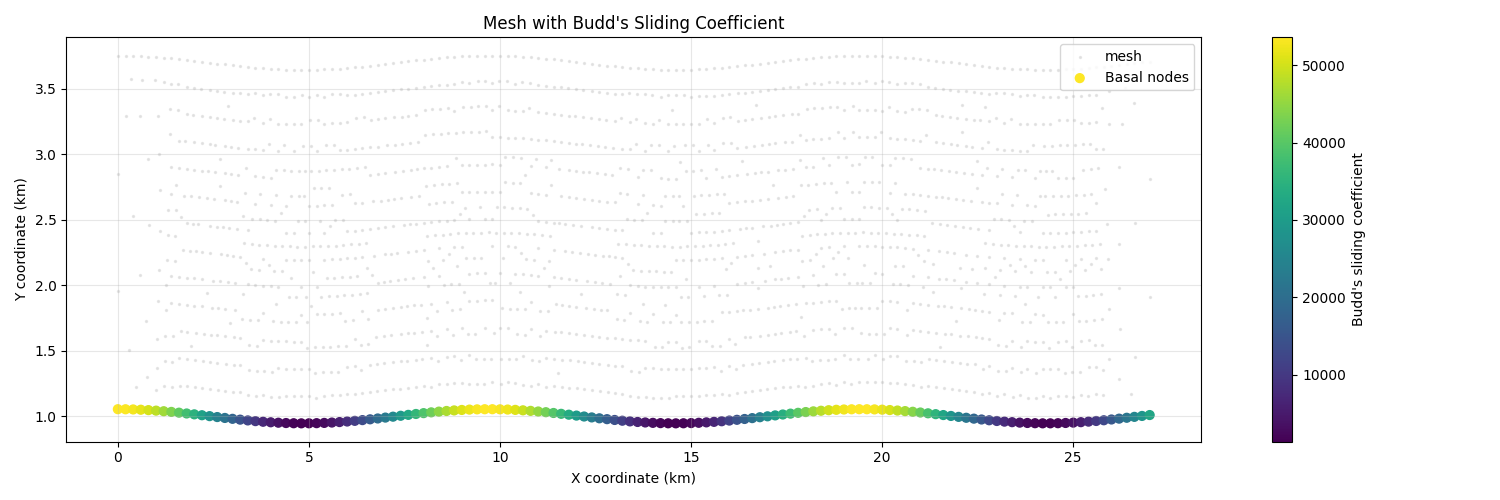
\includegraphics[scale=0.5]{basal_friction.png}
    \caption{Slope parallel visualisation of the computational mesh with basal nodes highlighted. The gray dotted lines represent the complete finite element mesh with multiple vertical layers conforming to the undulating geometry. Basal nodes (colored yellow to purple) follow the periodic bed topography with a wavelength of approximately 2.5 km, matching the dominant frequency observed in the filtered signals. The color gradient along the basal nodes may represent variations in basal friction coefficients implemented through Budd's sliding law, with darker colors potentially indicating regions of higher basal drag}
    \label{fig:Friction}
\end{figure}

\begin{figure}
    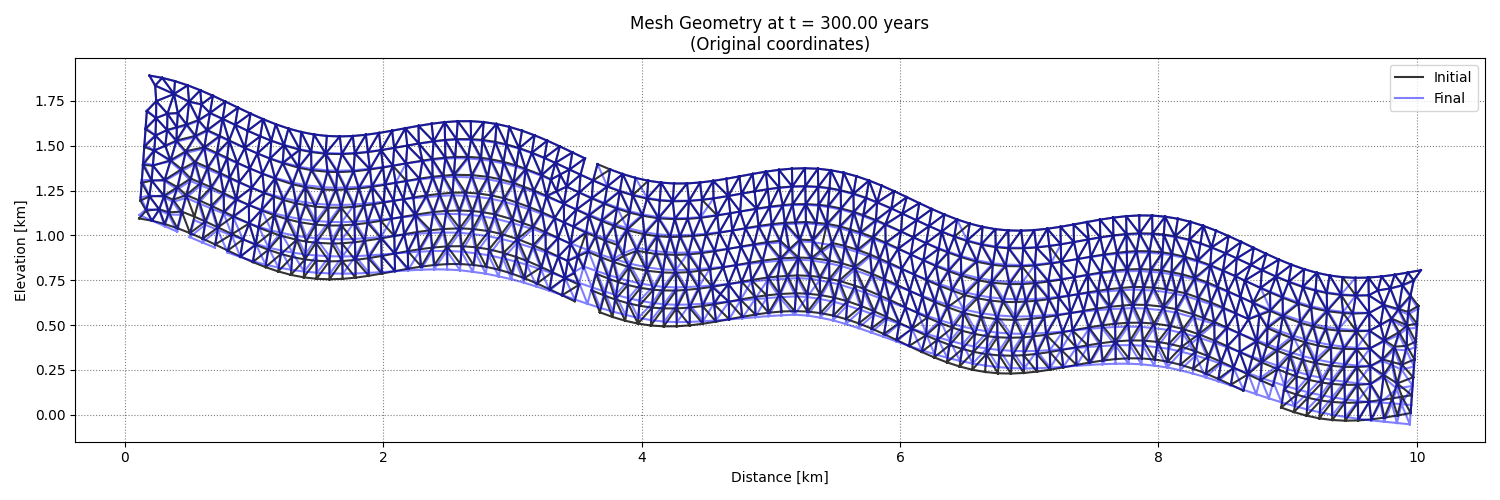
\includegraphics[scale=0.45]{overlap_xz.png}
    \caption{Mesh geometry evolution from initial state (black outline) to final configuration at t = 300.00 years (blue mesh) shown in original coordinates. The unstructured triangular finite element mesh adapts to the changing ice geometry while maintaining numerical stability. Presently both the surface and basal boundaries preserve the wavelength of the underlying bed topography ($\lambda = 2.64$ km), with similar amplitudes and phase relationships. This is not the expected result. The final mesh appears to be moved near the base when compared to the initial mesh setup. This demonstrates that there is a problem in the transient computation.}
    \label{fig:}
\end{figure}

\begin{figure}
    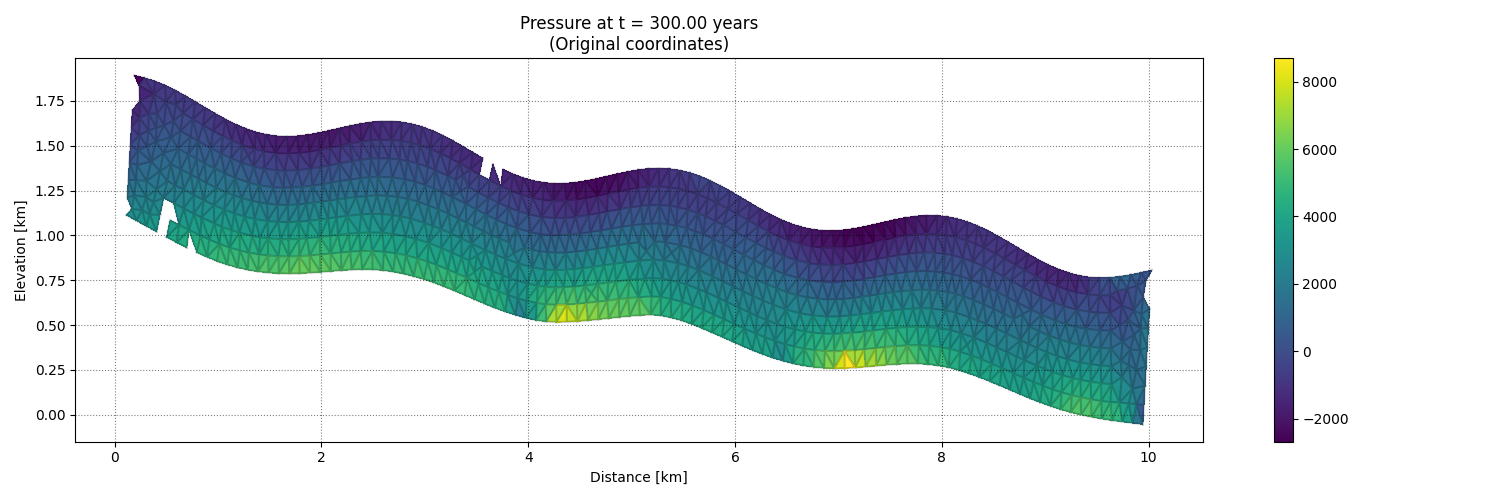
\includegraphics[scale=0.45]{Pressure_300yrs_xz.png}
    \caption{Pressure field distribution at t = 300.00 years shown in original coordinates. The color scale (ranging from -2000 to 8000 Pa) reveals the spatial pressure variations throughout the ice body, with higher pressures (yellow) concentrated near the peaks of the bed undulations as per Budd's sliding theory. The triangular mesh elements display the finite element discretisation used for solving the Stokes equations. Note the development of low-pressure zones (dark blue/purple) near the surface that align with the undulating basal topography, suggesting stress transfer from variation in basal friction. The asymmetric pressure distribution along the flow direction indicates the influence of the applied boundary conditions and developing stress regime within the ice.}
    \label{fig:}
\end{figure}

\begin{figure}
    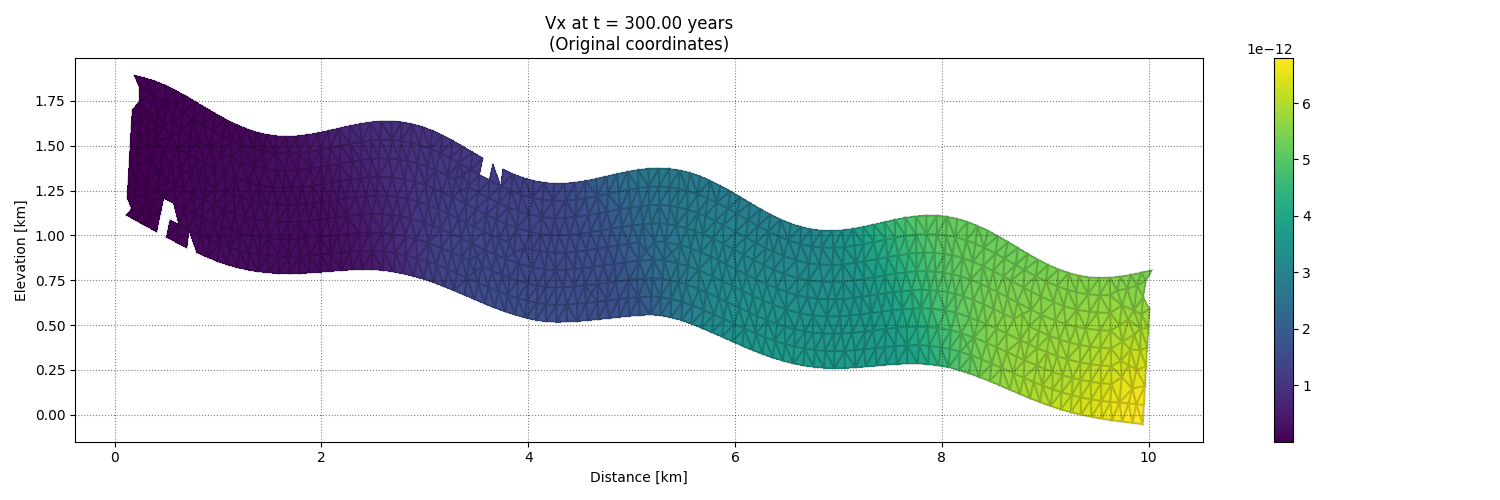
\includegraphics[scale=0.45]{Vx_300yrs_xz.png}
    \caption{Horizontal velocity field (Vx) at t = 300.00 years displayed in original coordinates. The color scale indicates velocity magnitude ($10^{-12}$ km/s, equivalent to $\approx 31.5$ mm/year at the maximum) with flow direction from left to right. The velocity pattern shows clear acceleration as the ice flows downslope, with highest velocities (yellow) occurring near the terminus. Note the velocity variations that correlate with the undulating bed topography implemented through the spatially varying basal friction coefficient in Budd's sliding law. The fixed upstream boundary condition (dark purple region at x=0) constrains flow at the inlet, while the progressive acceleration downstream results from gravitational forcing along the sloped bed}
    \label{fig:Vx}
\end{figure}

\begin{figure}
    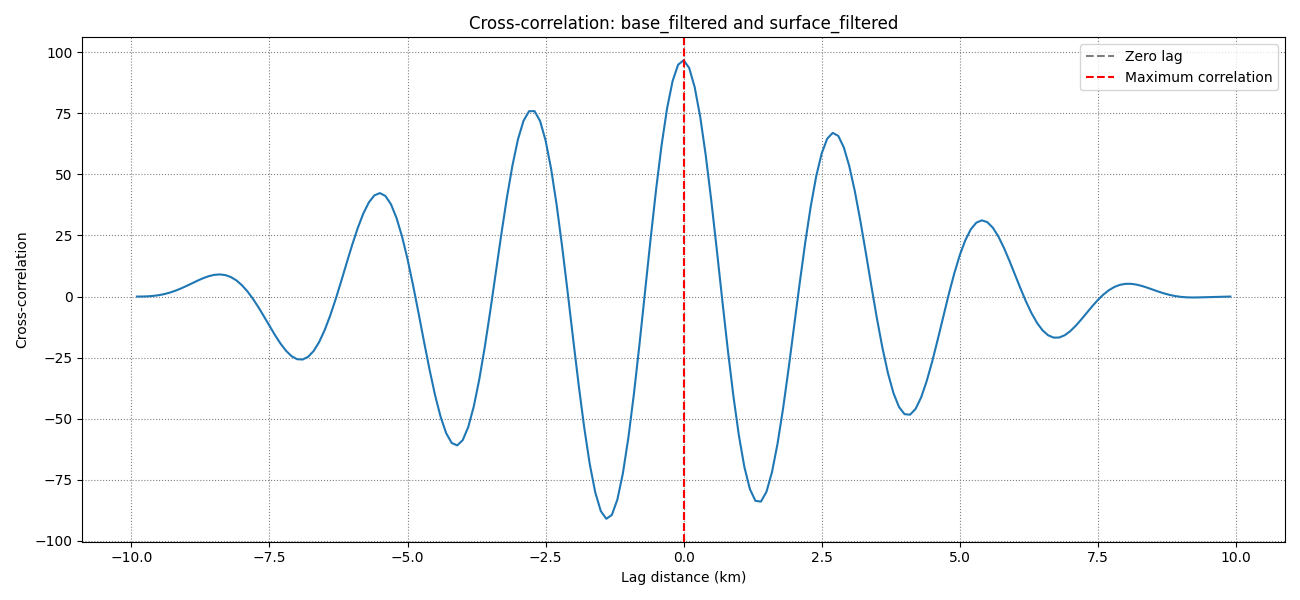
\includegraphics[scale=0.5]{xcorr_filtered.png}
    \caption{Cross-correlation between the filtered base and filtered surface signals across spatial lags. Maximum correlation of approximately 98\% occurs at zero lag, with periodic oscillations of decreasing amplitude at increasing distances. The symmetric pattern indicates similar signal structures in both datasets, with a characteristic wavelength of approximately 2.5 km between correlation peaks.}
    \label{fig:xcorr_filtered}
\end{figure}

\begin{figure}
    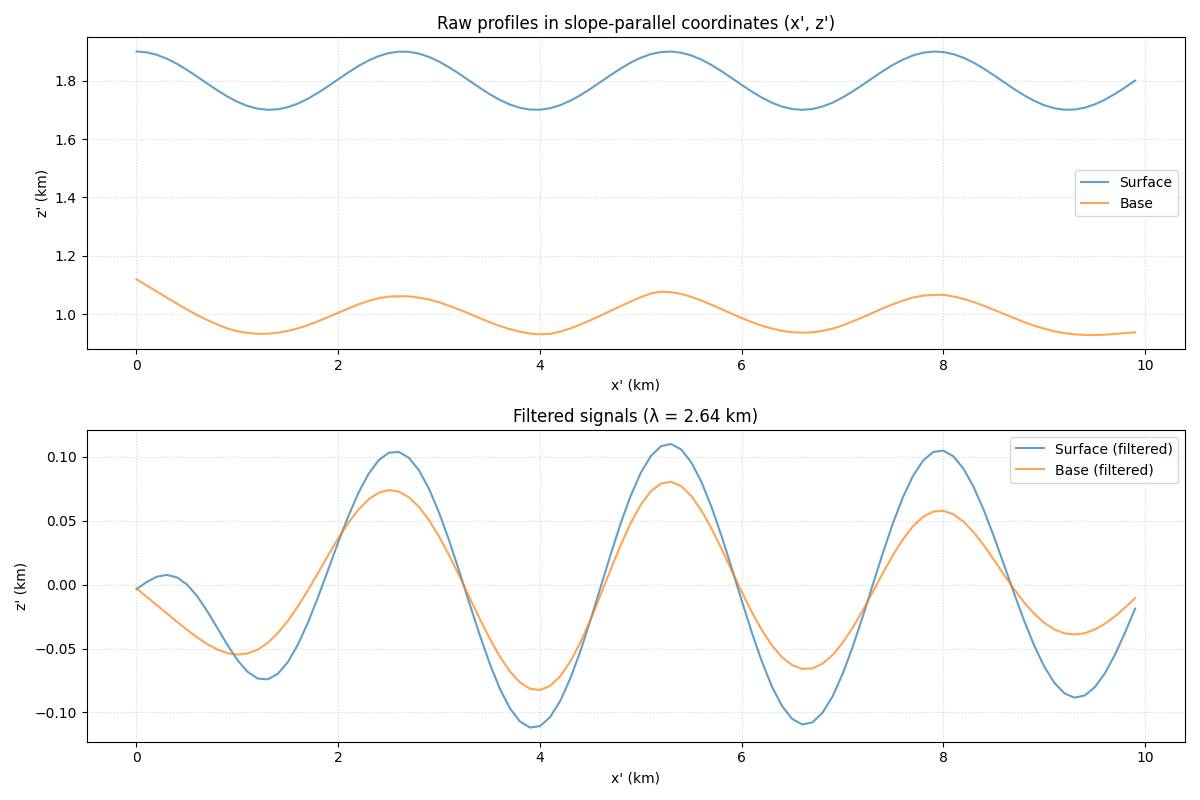
\includegraphics[scale=0.5]{base_surf_overlap.png}
    \caption{Topographic profiles and filtered signals in slope-parallel coordinates. Upper panel: Raw elevation profiles showing surface (blue) and base (orange) interfaces with periodic undulations along a 10 km domain. Lower panel: Filtered signals ($\lambda = 2.64$km) highlighting wavelength-specific components of surface and base topography after removing the mean trend, revealing strong spatial correlation in phase and amplitude. This implementation demonstrates how basal topography influences surface expression through a spatially varying basal friction governed by a simplified version of Budd's sliding law}
    \label{fig:overlap}
\end{figure}
